\documentclass[11pt,a4paper]{article}

\usepackage[margin=1in]{geometry}
\usepackage{booktabs}
\usepackage{graphicx}
\usepackage{amsmath}
\usepackage{hyperref}
\usepackage{caption}
\usepackage{float}
\usepackage{parskip}
\usepackage[T1]{fontenc}
\usepackage{lmodern}

\hypersetup{colorlinks=true, linkcolor=blue, urlcolor=blue}

\title{\textbf{Machine Learning Assignment 1}\\[0.4em]
       \large Polynomial Regression --- Steam Turbine Optimisation \& Thermal Reservoir Mapping}
\author{BT2024218}
\date{October 2026}

\begin{document}

\maketitle
\tableofcontents
\newpage

% ---------------------------------------------------------------
\section{Problem Overview}

Two polynomial regression problems are addressed, each with a personalised dataset.

\begin{itemize}
  \item \textbf{var1 -- Steam Turbine Optimisation:} Predict the Net Power Score $y$ from
        six operational parameters $(x_1,\ldots,x_6)$ using a polynomial of degree up to 10.
  \item \textbf{var2 -- Thermal Reservoir Mapping:} Predict the Thermal Anomaly Score $y$
        from three spatial coordinates $(x_1, x_2, x_3)$ using a polynomial of degree up to 20.
\end{itemize}

Both datasets are pre-cleaned. The target variable in every file is \texttt{y}.

% ---------------------------------------------------------------
\section{Methodology}

\subsection{General Pipeline}

For both problems the same five-step pipeline is applied:

\begin{enumerate}
  \item Split the training data into an 80\% development set and a 20\% hold-out set
        (fixed \texttt{random\_state=42}).
  \item For each candidate degree, fit a regularised polynomial model on the development
        set using 5-fold cross-validation to tune the regularisation strength.
        Record the mean CV MSE across folds at the best regularisation parameter.
  \item Select the degree with the lowest CV MSE.
  \item Evaluate the chosen degree \emph{once} on the untouched hold-out set (MSE, $R^2$).
  \item Refit on the full training data with the chosen degree and produce predictions for
        the test set.
\end{enumerate}

\subsection{Polynomial Feature Expansion}

Given input $\mathbf{x} \in \mathbb{R}^p$, polynomial features of degree $d$ generate all
monomials $x_1^{a_1} x_2^{a_2} \cdots x_p^{a_p}$ with $\sum_i a_i \leq d$.
The expanded features are standardised (zero mean, unit variance) before fitting.

\subsection{Regularisation Strategy}

\paragraph{var1 --- Lasso (L1).}
With $p=6$ features and degree up to 10, the expanded feature space can exceed several
thousand terms.  Lasso's L1 penalty drives irrelevant coefficients to exactly zero,
performing automatic feature selection and preventing overfitting.
The regularisation parameter $\alpha$ is chosen by \texttt{LassoCV} over a log-spaced
grid of 20 values.

\paragraph{var2 --- Ridge (L2).}
With only $p=3$ features the polynomial expansion remains manageable even at degree 20.
Ridge's L2 penalty shrinks all coefficients smoothly without zeroing them, which suits
the smooth geological surface being modelled.
The regularisation parameter $\alpha$ is chosen by \texttt{RidgeCV} over a log-spaced
grid of 40 values ranging from $10^{-6}$ to $10^{4}$.

% ---------------------------------------------------------------
\section{Phase 1 -- Steam Turbine Optimisation (var1)}

\subsection{Dataset}
Training: 1000 samples, 6 features. Test: 1000 samples.

\subsection{Degree Selection}

\begin{table}[H]
  \centering
  \caption{var1: CV MSE and hold-out metrics for each polynomial degree (Lasso).}
  \label{tab:var1}
  \begin{tabular}{rrrr}
    \toprule
    \textbf{Degree} & \textbf{CV MSE} & \textbf{Hold-out MSE} & \textbf{Hold-out $R^2$} \\
    \midrule
    1  & 9.0011 & 8.1066 & 0.1166 \\
    2  & 3.1111 & 2.7741 & 0.6977 \\
    3  & 1.0760 & 0.9165 & 0.9001 \\
    4  & 0.7242 & 0.6029 & 0.9343 \\
    \textbf{5}  & \textbf{0.3467} & \textbf{0.3590} & \textbf{0.9609} \\
    6  & 0.3679 & 0.3637 & 0.9604 \\
    7  & 0.3865 & 0.3818 & 0.9584 \\
    8  & 0.3941 & 0.3758 & 0.9591 \\
    9  & 0.3994 & 0.3788 & 0.9587 \\
    10 & 0.4037 & 0.3816 & 0.9584 \\
    \bottomrule
  \end{tabular}
\end{table}

\subsection{Analysis}

The CV MSE decreases steeply from degree 1 to 5 and then rises monotonically from
degree 6 onward (Figure~\ref{fig:var1}), indicating overfitting beyond degree 5.
\textbf{Degree 5} is selected as the optimal degree.

On the held-out 20\%:
\[
  \text{MSE} = 0.3590, \qquad R^2 = 0.9609
\]

\begin{figure}[H]
  \centering
  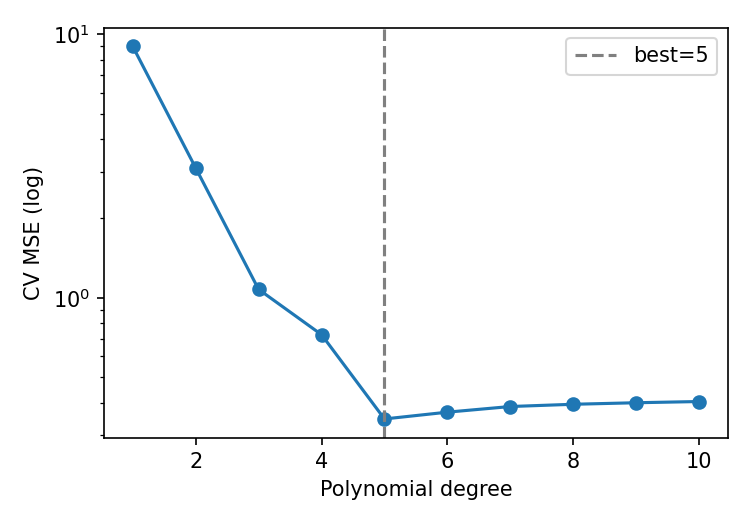
\includegraphics[width=0.6\textwidth]{part1_cv_curve.png}
  \caption{var1: CV MSE vs.\ polynomial degree. The dashed line marks degree 5.}
  \label{fig:var1}
\end{figure}

% ---------------------------------------------------------------
\section{Phase 2 -- Thermal Reservoir Mapping (var2)}

\subsection{Dataset}
Training: 1000 samples, 3 features. Test: 1000 samples.

\subsection{Degree Selection}

\begin{table}[H]
  \centering
  \caption{var2: CV MSE and hold-out metrics for each polynomial degree (Ridge).}
  \label{tab:var2}
  \begin{tabular}{rrrr}
    \toprule
    \textbf{Degree} & \textbf{CV MSE} & \textbf{Hold-out MSE} & \textbf{Hold-out $R^2$} \\
    \midrule
    1  & 39.4143 & 25.1706 & 0.2779 \\
    2  & 23.4251 & 17.8965 & 0.4866 \\
    3  & 12.9633 &  8.6325 & 0.7523 \\
    4  &  4.2470 &  2.9721 & 0.9147 \\
    5  &  1.7873 &  1.2768 & 0.9634 \\
    6  &  0.6090 &  0.5482 & 0.9843 \\
    7  &  0.3764 &  0.3686 & 0.9894 \\
    8  &  0.2618 &  0.3108 & 0.9911 \\
    9  &  0.2677 &  0.3013 & 0.9914 \\
    \textbf{10} & \textbf{0.2534} & \textbf{0.2905} & \textbf{0.9917} \\
    11 &  0.2600 &  0.2923 & 0.9916 \\
    12 &  0.2592 &  0.2907 & 0.9917 \\
    13 &  0.2671 &  0.2954 & 0.9915 \\
    14 &  0.2737 &  0.2936 & 0.9916 \\
    15 &  0.2807 &  0.2993 & 0.9914 \\
    16 &  0.2904 &  0.3047 & 0.9913 \\
    17 &  0.2965 &  0.3106 & 0.9911 \\
    18 &  0.3074 &  0.3135 & 0.9910 \\
    19 &  0.3139 &  0.3186 & 0.9909 \\
    20 &  0.3277 &  0.3227 & 0.9907 \\
    \bottomrule
  \end{tabular}
\end{table}

\subsection{Analysis}

CV MSE decreases from degree 1 to 10 and begins to increase from degree 11
(Figure~\ref{fig:var2}), consistent with a complex but smooth thermal surface.
\textbf{Degree 10} is selected as the optimal degree.

On the held-out 20\%:
\[
  \text{MSE} = 0.2905, \qquad R^2 = 0.9917
\]

\begin{figure}[H]
  \centering
  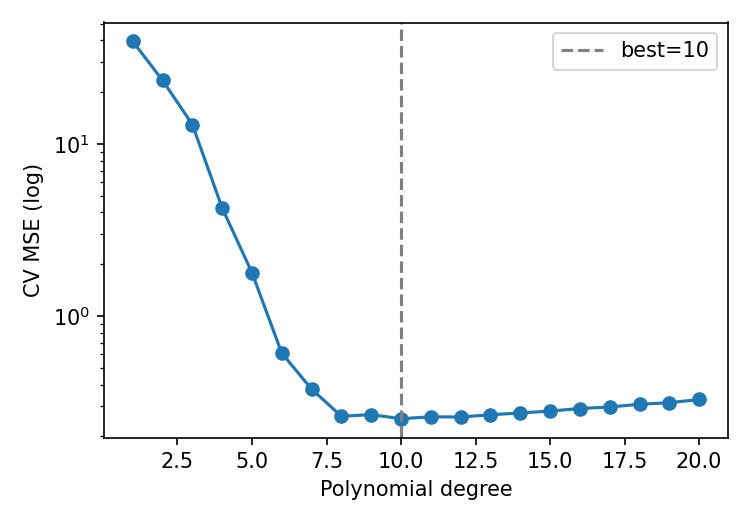
\includegraphics[width=0.6\textwidth]{part2_cv_curve.png}
  \caption{var2: CV MSE vs.\ polynomial degree. The dashed line marks degree 10.}
  \label{fig:var2}
\end{figure}

% ---------------------------------------------------------------
\section{Summary}

\begin{table}[H]
  \centering
  \caption{Final model summary.}
  \begin{tabular}{lcccc}
    \toprule
    \textbf{Problem} & \textbf{Regulariser} & \textbf{Best Degree} & \textbf{Hold-out MSE} & \textbf{Hold-out $R^2$} \\
    \midrule
    var1 (Steam Turbine)     & Lasso & 5  & 0.3590 & 0.9609 \\
    var2 (Thermal Reservoir) & Ridge & 10 & 0.2905 & 0.9917 \\
    \bottomrule
  \end{tabular}
\end{table}

Both models achieve $R^2 > 0.96$, indicating strong generalisation on the hold-out data.
The degree selection was driven entirely by cross-validated MSE with no look-ahead into
the test set.

% ---------------------------------------------------------------
\section{Submission Files}

\begin{itemize}
  \item \texttt{BT2024218\_pred\_var1.csv} --- 1000 predicted Net Power Scores.
  \item \texttt{BT2024218\_pred\_var2.csv} --- 1000 predicted Thermal Anomaly Scores.
  \item \texttt{part1.py} --- training and inference code for var1.
  \item \texttt{part2.py} --- training and inference code for var2.
\end{itemize}

\end{document}
